\section{Hierarchical clustering and ordered heatmaps}
\label{sec:clustering}

\subsection{Ordered heatmaps}

RMT separates the matrix into spectral components, but heatmaps help determine whether these components have visible block structure. Figure~\ref{fig:ordered_heatmaps} orders the assets through hierarchical clustering and displays original, filtered and group-mode structures. The purpose is visual and diagnostic: the heatmaps show whether the spectral filtering produces economically interpretable blocks rather than only abstract eigenvalue differences.

\begin{figure}
\centering
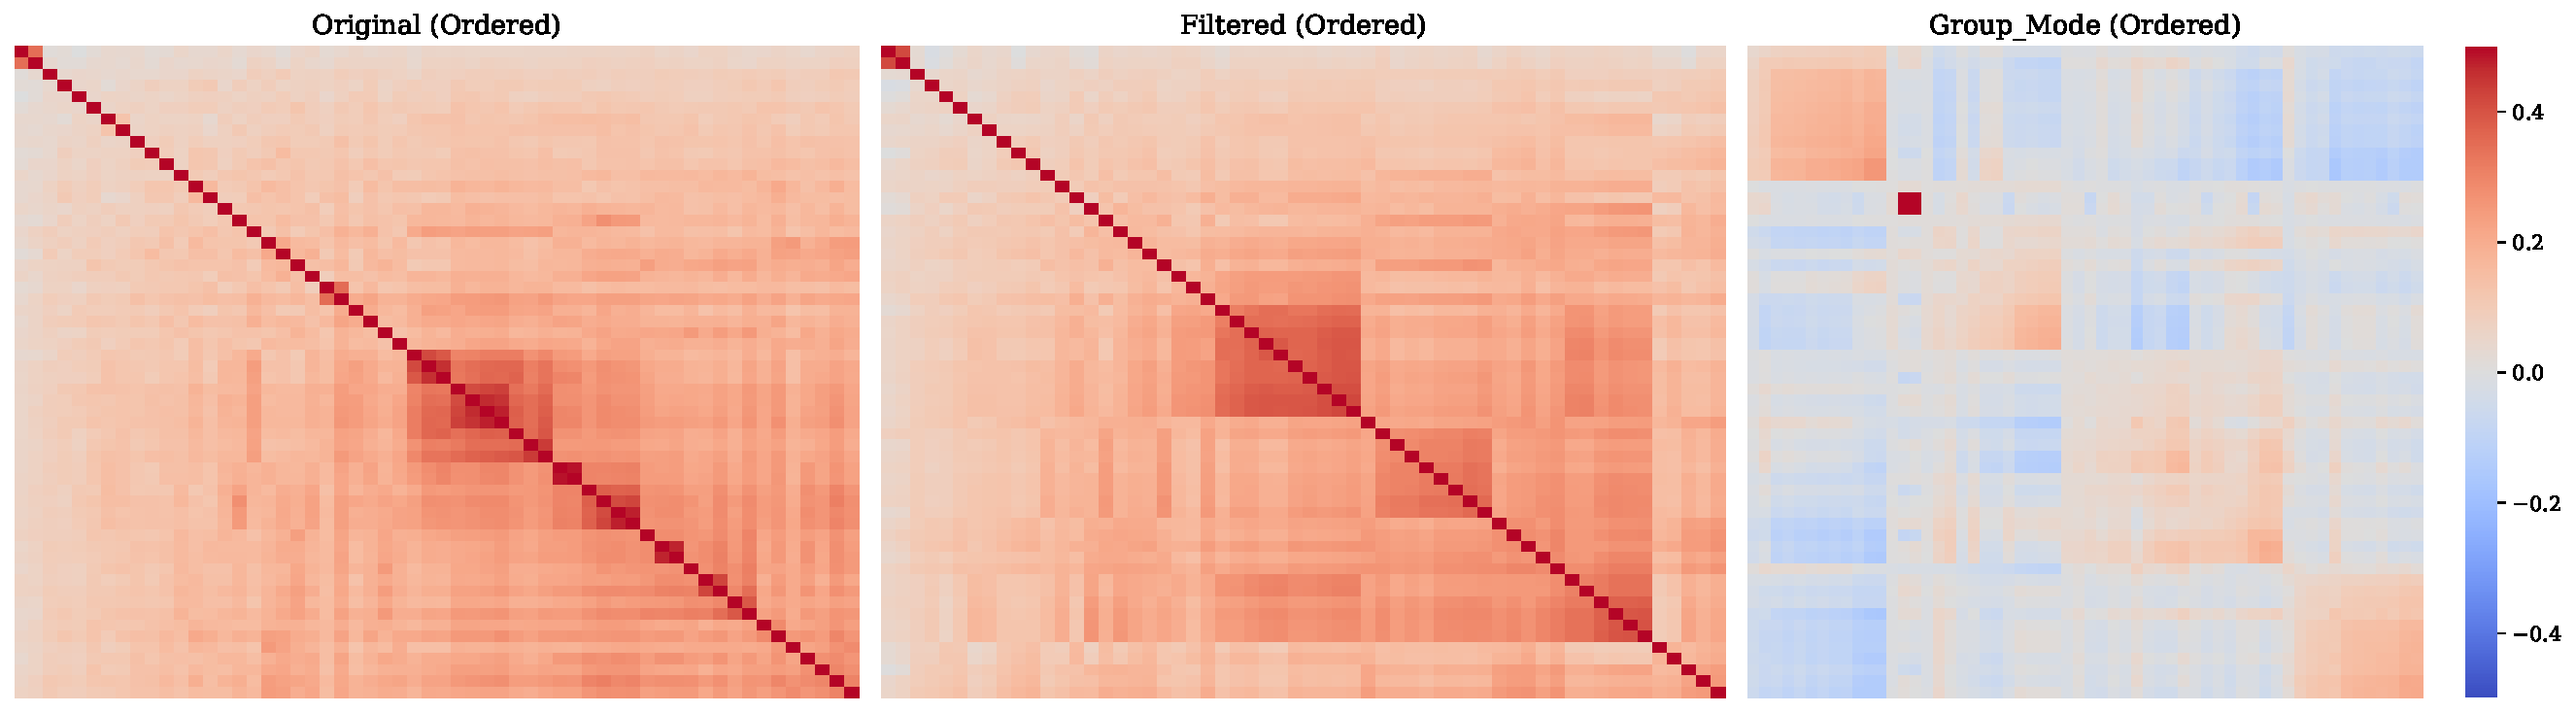
\includegraphics[width=\linewidth,height=0.78\textheight,keepaspectratio]{images/figure_10_ordered_heatmaps.pdf}
\caption{Ordered heatmaps for original and RMT-filtered correlation matrices. Hierarchical ordering reveals block structures that are less visible in unordered matrices.}
\label{fig:ordered_heatmaps}
\end{figure}
\FloatBarrier

The original matrix shows a broad positive background, consistent with the strong market mode. The filtered matrix preserves much of the organized dependency while suppressing noise. The group-mode heatmap is weaker in average correlation but more informative for localized blocks, because the dominant common component no longer masks sectoral variation. This is the visual counterpart of the RMT decomposition.

\subsection{Dendrograms comparison}

Dendrograms provide a complementary view of the same distance geometry. Figure~\ref{fig:dendrograms} compares hierarchical clustering trees for original, filtered and group-mode matrices. These trees help identify which assets join early, which branches are stable and how the removal of the market mode changes the hierarchy.

\begin{figure}
\centering
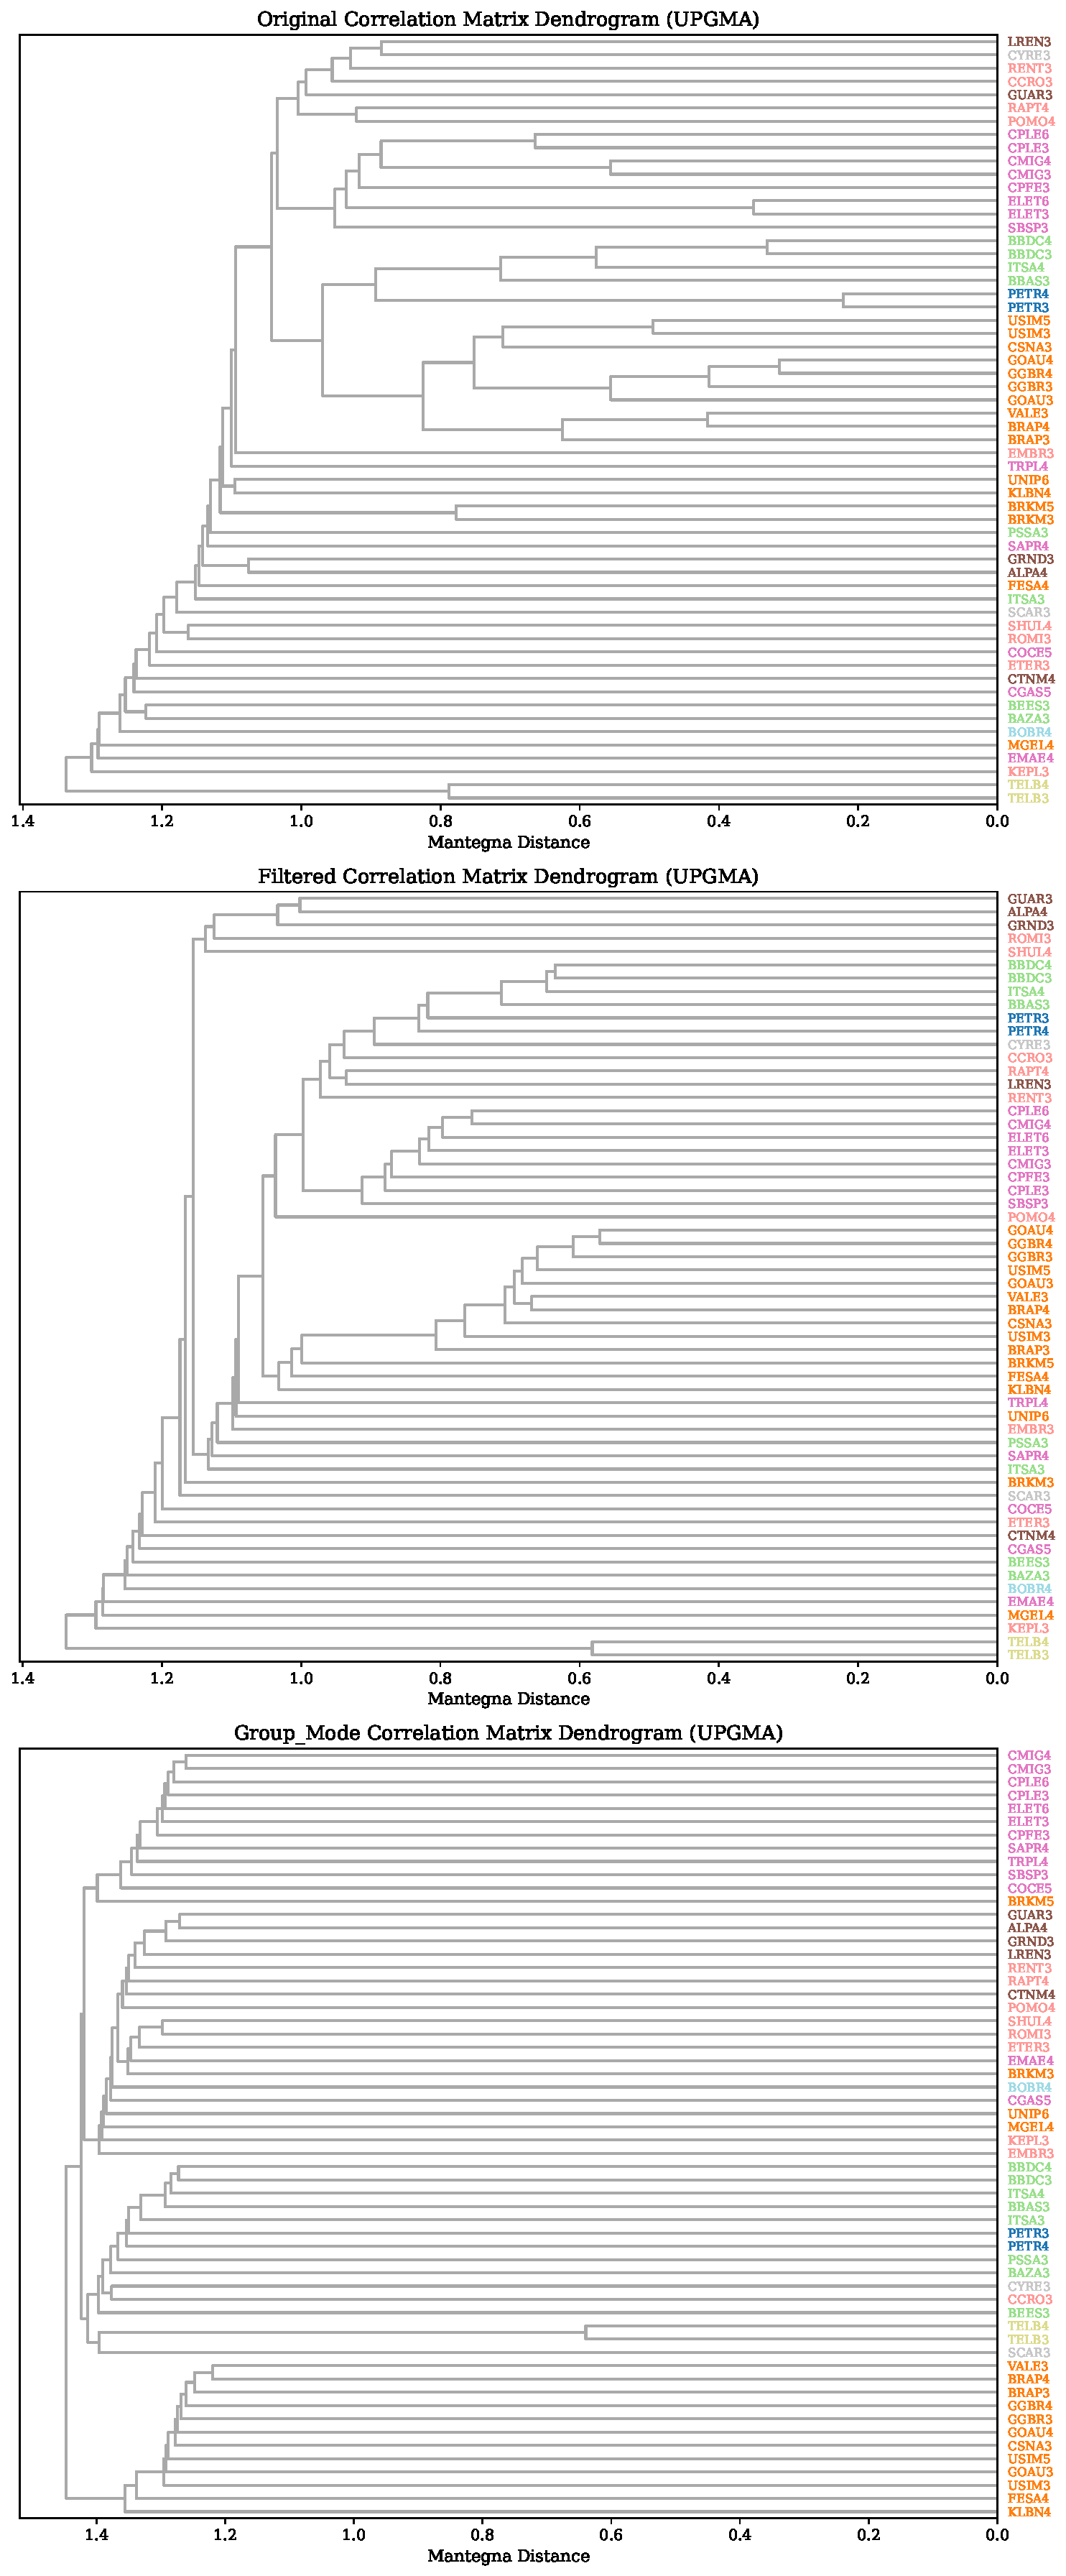
\includegraphics[width=\linewidth,height=0.78\textheight,keepaspectratio]{images/figure_9_dendrograms_comparison.pdf}
\caption{Dendrogram comparison for original, filtered and group-mode matrices using Mantegna distances and average linkage.}
\label{fig:dendrograms}
\end{figure}
\FloatBarrier

\begin{table}
\centering
\caption{Cophenetic correlations for hierarchical clustering.}
\label{tab:cophenetic_summary}
\begin{tabular}{lrr}
\toprule
Matrix & Assets & Cophenetic correlation \\
\midrule
Original & 58 & 0.9500 \\
Filtered & 58 & 0.9340 \\
Group Mode & 58 & 0.8705 \\
\bottomrule
\end{tabular}
\end{table}
\FloatBarrier

The cophenetic correlation is highest for the original matrix, 0.9500, and remains high for the filtered matrix, 0.9340. The group-mode value is lower, 0.8705. This decline is expected rather than problematic. Removing the market mode reduces the smooth common structure that makes the hierarchy easier to summarize, leaving a more localized and less homogeneous dependency system.

The clustering results connect naturally to network filtering. Ordered heatmaps and dendrograms show that localized structure survives RMT filtering. The next section asks how that structure appears when only the strongest distance-ranked edges are retained under MST and PMFG constraints.
